% !TEX TS-program = knitr
\documentclass{article}\usepackage{graphicx, color}
%% maxwidth is the original width if it is less than linewidth
%% otherwise use linewidth (to make sure the graphics do not exceed the margin)
\makeatletter
\def\maxwidth{ %
  \ifdim\Gin@nat@width>\linewidth
    \linewidth
  \else
    \Gin@nat@width
  \fi
}
\makeatother

\IfFileExists{upquote.sty}{\usepackage{upquote}}{}
\definecolor{fgcolor}{rgb}{0.2, 0.2, 0.2}
\newcommand{\hlnumber}[1]{\textcolor[rgb]{0,0,0}{#1}}%
\newcommand{\hlfunctioncall}[1]{\textcolor[rgb]{0.501960784313725,0,0.329411764705882}{\textbf{#1}}}%
\newcommand{\hlstring}[1]{\textcolor[rgb]{0.6,0.6,1}{#1}}%
\newcommand{\hlkeyword}[1]{\textcolor[rgb]{0,0,0}{\textbf{#1}}}%
\newcommand{\hlargument}[1]{\textcolor[rgb]{0.690196078431373,0.250980392156863,0.0196078431372549}{#1}}%
\newcommand{\hlcomment}[1]{\textcolor[rgb]{0.180392156862745,0.6,0.341176470588235}{#1}}%
\newcommand{\hlroxygencomment}[1]{\textcolor[rgb]{0.43921568627451,0.47843137254902,0.701960784313725}{#1}}%
\newcommand{\hlformalargs}[1]{\textcolor[rgb]{0.690196078431373,0.250980392156863,0.0196078431372549}{#1}}%
\newcommand{\hleqformalargs}[1]{\textcolor[rgb]{0.690196078431373,0.250980392156863,0.0196078431372549}{#1}}%
\newcommand{\hlassignement}[1]{\textcolor[rgb]{0,0,0}{\textbf{#1}}}%
\newcommand{\hlpackage}[1]{\textcolor[rgb]{0.588235294117647,0.709803921568627,0.145098039215686}{#1}}%
\newcommand{\hlslot}[1]{\textit{#1}}%
\newcommand{\hlsymbol}[1]{\textcolor[rgb]{0,0,0}{#1}}%
\newcommand{\hlprompt}[1]{\textcolor[rgb]{0.2,0.2,0.2}{#1}}%

\usepackage{framed}
\makeatletter
\newenvironment{kframe}{%
 \def\at@end@of@kframe{}%
 \ifinner\ifhmode%
  \def\at@end@of@kframe{\end{minipage}}%
  \begin{minipage}{\columnwidth}%
 \fi\fi%
 \def\FrameCommand##1{\hskip\@totalleftmargin \hskip-\fboxsep
 \colorbox{shadecolor}{##1}\hskip-\fboxsep
     % There is no \\@totalrightmargin, so:
     \hskip-\linewidth \hskip-\@totalleftmargin \hskip\columnwidth}%
 \MakeFramed {\advance\hsize-\width
   \@totalleftmargin\z@ \linewidth\hsize
   \@setminipage}}%
 {\par\unskip\endMakeFramed%
 \at@end@of@kframe}
\makeatother

\definecolor{shadecolor}{rgb}{.97, .97, .97}
\definecolor{messagecolor}{rgb}{0, 0, 0}
\definecolor{warningcolor}{rgb}{1, 0, 1}
\definecolor{errorcolor}{rgb}{1, 0, 0}
\newenvironment{knitrout}{}{} % an empty environment to be redefined in TeX

\usepackage{alltt}

\usepackage{amsfonts}
\usepackage{amsmath}
\usepackage{amssymb}
\usepackage{amsthm}
\usepackage{caption}
\usepackage{color}
\usepackage{enumerate}
\usepackage{fancyhdr}
\usepackage{hyperref}
\usepackage{graphicx}
\usepackage{latexsym}
\usepackage{listings}
\usepackage{mathrsfs}
\usepackage{natbib}
\usepackage[nottoc]{tocbibind}
\usepackage{url}

\providecommand{\all}{\ \forall \ }
\providecommand{\bs}{\backslash}
\providecommand{\e}{\varepsilon}
\providecommand{\E}{\ \exists \ }
\providecommand{\lm}[2]{\lim_{#1 \rightarrow #2}}
\providecommand{\m}[1]{\mathbb{#1}}
\providecommand{\nv}{{}^{-1}}
\providecommand{\ov}[1]{\overline{#1}}
\providecommand{\p}{\newpage}
\providecommand{\q}{$\quad$ \newline}
\providecommand{\rt}{\rightarrow}
\providecommand{\Rt}{\Rightarrow}
\providecommand{\vc}[1]{\boldsymbol{#1}}
\providecommand{\wh}[1]{\widehat{#1}}

%\renewcommand\bibname{References}
%\renewcommand{\thesection}{Problem \arabic{section}}
%\renewcommand{\thesubsection}{Part \alph{subsection}}
\numberwithin{equation}{section}

\fancyhead{}
\fancyfoot{}
\fancyhead[R]{\thepage}
\fancyhead[C]{Landau}

\hypersetup{
    colorlinks,
    citecolor=black,
    filecolor=black,
    linkcolor=black,
    urlcolor=blue
}

\definecolor{dkgreen}{rgb}{0,0.6,0}
\definecolor{gray}{rgb}{0.5,0.5,0.5}
\definecolor{mauve}{rgb}{0.58,0,0.82}

\lstset{ 
  language=C,                % the language of the code
  basicstyle=\Large,           % the size of the fonts that are used for the code
  numberstyle= \tiny \color{white},  % the style that is used for the line-numbers
  stepnumber=2,                   % the step between two line-numbers. 
  numbersep=5pt,                  % how far the line-numbers are from the code
  backgroundcolor=\color{white},      % choose the background color. You must add \usepackage{color}
  showspaces=false,               % show spaces adding particular underscores
  showstringspaces=false,         % underline spaces within strings
  showtabs=false,                 % show tabs within strings adding particular underscores
  frame=lrb,                   % adds a frame around the code
  rulecolor=\color{black},        % if not set, the frame-color may be changed on line-breaks within not-black text 
  tabsize=2,                      % sets default tabsize to 2 spaces
  captionpos=t,                   % sets the caption-position 
  breaklines=true,                % sets automatic line breaking
  breakatwhitespace=false,        % sets if automatic breaks should only happen at whitespace
  title=\lstname,                   % show the filename of files included with \lstinputlisting;
  keywordstyle=\color{blue},          % keyword style
  commentstyle=\color{gray},       % comment style
  stringstyle=\color{dkgreen},         % string literal style
  escapeinside={\%*}{*)},            % if you want to add LaTeX within your code
  morekeywords={*, ...},               % if you want to add more keywords to the set
  xleftmargin=0.053in, % left horizontal offset of caption box
  xrightmargin=-.03in % right horizontal offset of caption box
}

\DeclareCaptionFont{white}{\color{white}}
\DeclareCaptionFormat{listing}{\parbox{\textwidth}{\colorbox{gray}{\parbox{\textwidth}{#1#2#3}}\vskip-0.05in}}
\captionsetup[lstlisting]{format = listing, labelfont = white, textfont = white}
% For caption-free listings, comment out the 3 lines above and uncomment the 2 lines below.
% \captionsetup{labelformat = empty, labelsep = none}
% \lstset{frame = single}






\begin{document}



\begin{flushleft}


\begin{center} \LARGE
STAT 305 D Homework 2 Solutions
\end{center}
\begin{center} \Large
Due January 31, 2012 at 12:40 PM in class
\end{center}


\begin{enumerate}[1. ]
\item Vardeman and Jobe Chapter 1 Exercise 2 (page 23): If factor A has levels 1, 2, and 3, factor B has levels 1 and 2, and factor C has levels 1 and 2, list the combinations of A, B, and C that make up a full factorial arrangement.

\color{red}
You can list all the combinations in a table: 

\begin{center}
\begin{tabular}{ccc}
A & B & C \\ \hline
1 & 1 & 1 \\ 
1 & 1 & 2 \\ 
1 & 2 & 1 \\ 
1 & 2 & 2 \\ 
2 & 1 & 1 \\ 
2 & 1 & 2 \\ 
2 & 2 & 1 \\ 
2 & 2 & 2 \\ 
3 & 1 & 1 \\ 
3 & 1 & 2 \\ 
3 & 2 & 1 \\ 
3 & 2 & 2 \\ 
\end{tabular}
\end{center}

\color{black}


\item Vardeman and Jobe Chapter 1 Exercise 10 (page 24): Give an example of a 2 $\times$ 3 full factorial data structure that might arise in a student study of the breaking strengths of wooden dowels. (Name the two factors involved, their levels, and write out all six different combinations. You must create the factors yourself. They are not given to you in this problem.) Then make up a data collection form for the study. Plan to record both the breaking strength and whether the break was clean or splintered for each dowel, supposing that three dowels of each type are to be tested.


\color{red}

In a factorial study, the factors are treatments, not blocks. Hence, I must choose factors that describe things that the experimenter does to the dowels. Humidity with levels high, medium, and low is a treatment factor because I can subject dowels to different humidities during the two weeks before testing breaking strength. I can also choose whether or not to soak them in water the day before the test, which gives me another treatment factor with two levels (soak or not soak). \q

Here is a corresponding data collection form if I assign one dowel per combination of treatment levels:

\begin{center}
\begin{tabular}{cccc}
Humidity & Soak? & Breaking strength & Clean break? \\ \hline
High & Yes &  &  \\ 
High & No &  &  \\ 
Med & Yes &  &  \\ 
Med & No &  &  \\ 
Low & Yes &  &  \\ 
Low & No &  &  \\ 
\end{tabular}
\end{center}

Since I haven't carried out the experiment yet, I'm leaving the last two columns blank. You could have also filled them with hypothetical data, but just be aware that you don't actually know what the breaking strengths and kinds of break will be until you apply the treatments and do the experiment. \q

The above data collection form has only one row per treatment combination, so there is only one dowel per treatment group. A better data collection form would thus allow for more than one dowel per treatment group: i.e., multiple \emph{replicates}:

\begin{center}
\begin{tabular}{cccc}
Humidity & Soak? & Breaking strength & Clean break? \\ \hline
High & Yes &  &  \\ 
High & Yes &  &  \\ 
High & Yes &  &  \\ 
High & No &  &  \\ 
High & No &  &  \\ 
High & No &  &  \\ 
Med & Yes &  &  \\ 
Med & Yes &  &  \\ 
Med & Yes &  &  \\ 
Med & No &  &  \\ 
Med & No &  &  \\ 
Med & No &  &  \\ 
Low & Yes &  &  \\
Low & Yes &  &  \\
Low & Yes &  &  \\
Low & No &  &  \\ 
Low & No &  &  \\  
Low & No &  &  \\ 
\end{tabular}
\end{center}

\color{black}


\item  Vardeman and Jobe Chapter 2 Exercise 3 (page 64): 

An experiment is to be performed to compare the effects of two different methods for loading gears in a carburizing furnace on the amount of distortion produced in a heat treating process. Thrust face runout will be measured for gears laid and for gears hung while treating.

\begin{enumerate}[a. ]
\item 20 gears are to be used in the study. Randomly divide up the gears into a group (of 10) to be laid and a group (of 10) to be hung, using Table B.1 (available at \href{http://will-landau.com/stat305/tables/random-digits.pdf}{http://will-landau.com/stat305/tables/random-digits.pdf}). Describe carefully how you do this. If you use the table, begin in the upper left corner.

\color{red}

First, I give each of the 20 gears and 2-digit index from 00 to 19. I move along the random number table, starting at the top left: \q

\setkeys{Gin}{width=1\textwidth} 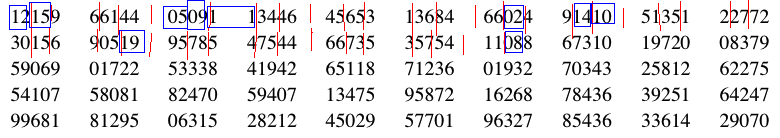
\includegraphics{../../fig/h2p3tab.png} 


I pick the first 10 of these indices I encounter: 12, 15, 05, 09, 11, 02, 14, 10, 19, and 08, which are shown in blue. I assign these gears to be laid. I assign the rest to be hung.


\color{black}



\item What are some purposes of the randomization used in part (a)? \q


\color{red}
The purpose of randomization is to make sure that there is no systematic difference between the treatment groups before a treatment is applied. That way, we can be reasonably sure that all the systematic differences between the treatment groups that we see after the experiment were caused by the treatment. 
\color{black}



\end{enumerate}


\item Now, suppose you want to distinguish between the big gears (10 of them) and the small gears (10 of them). You want to design an improved study to test the effect of gear arrangement on gear distortion. This new study takes the different gear sizes into account. (After all, small gears may distort less than big gears, or vice versa.) You plan to lay 5 small gears, hang 5 small gears, lay 5 big gears, and hang 5 big gears.

\begin{enumerate}[a. ]
\item Name the design of the study. Also, construct a table with all sample units as rows and variables as columns to show all the combinations of levels of the variables.

\color{red}

This is a randomized complete block design with gear arrangement as a treatment variable and gear size as the blocking variable. The table looks like this:

\begin{tabular}{ccc}

Gear size & Gear arrangement & Distortion  \\ \hline
Big & Laid &  \\ 
Big & Laid &  \\ 
Big & Laid &  \\ 
Big & Laid &  \\ 
Big & Laid &  \\ 
Big & Hung &  \\ 
Big & Hung &  \\ 
Big & Hung &  \\ 
Big & Hung &  \\ 
Big & Hung &  \\ 
Small & Laid & \\
Small & Laid & \\
Small & Laid & \\
Small & Laid & \\
Small & Laid & \\
Small & Hung & \\
Small & Hung & \\
Small & Hung & \\
Small & Hung & \\
Small & Hung & \\
\end{tabular} \q

I haven't done the experiment, so I leave the gear distortion column blank. I didn't even need to include that column, but I include it to show that, since there is one gear per row, I record one distortion measurement per row during the experiment.

\color{black}




\item Carry out the appropriate randomization to assign the 20 gears to the appropriate treatment groups for the experiment.
\end{enumerate}


\color{red}

Since this is a randomized complete block design, I randomize gears to treatment groups \emph{within each block}. That means I first randomize the small gears to be laid or hung, and then I randomize the big gears to be laid or hung.

\begin{enumerate}[i. ]
\item Big gears: \q

I assign each of the big gears an index from 0 to 9. Starting at the top left corner of the random number table, I move along the random digits, picking the first unique five I see to be laid: \q

\setkeys{Gin}{width=1\textwidth} 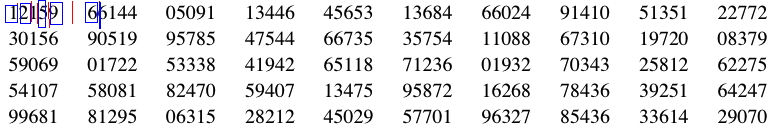
\includegraphics{../../fig/h2p4tab1.png}

As I show with blue boxes, I pick big gears 1, 2, 5, 9, and 6 to be laid. I pick the rest to be hung.

\item Small gears: \q

I assign each of the small gears an index from 0 to 9. Then, picking up where I left off in the random number table, I move along the random digits, picking the first unique five I see to be laid: \q


\setkeys{Gin}{width=1\textwidth} 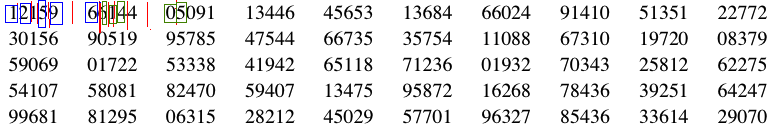
\includegraphics{../../fig/h2p4tab2.png}

As I show with green boxes, I pick small gears 6, 1, 4, 0, and 5 to be laid. I pick the rest to be hung. \q

Note that it's important to continue where you left off in the random number table from the big gears when you randomize the small gears. If you start from the top left corner for each, you will pick big gears 1, 2, 5, 9, and 6 to be laid and small gears 1, 2, 5, 9, and 6 to be laid. Instead, I want to randomize the big gears independently of the small gears.

\end{enumerate}

\color{black}



\item Vardeman and Jobe Chapter 3 Section 1 problem 1 (page 77):

\setkeys{Gin}{width=.75\textwidth} 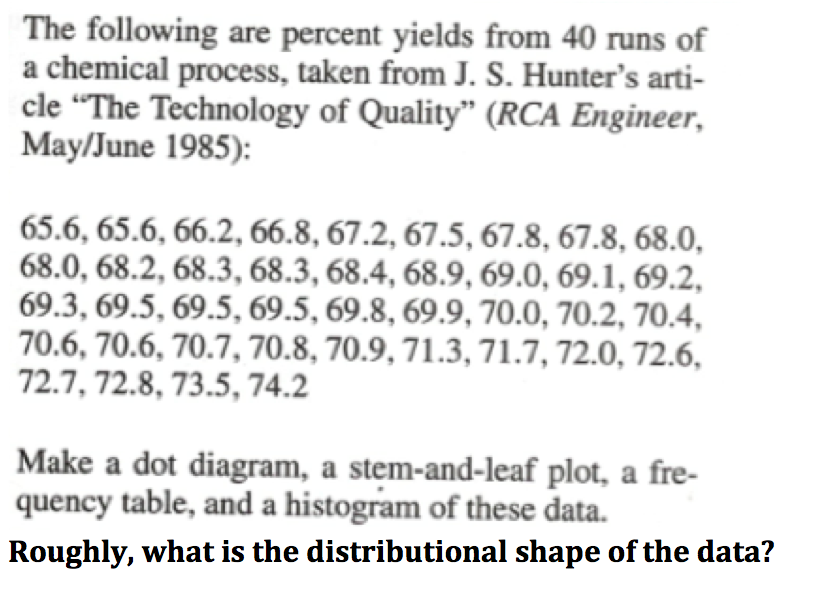
\includegraphics{../../fig/ch3s1p1.png}

\setkeys{Gin}{width=1\textwidth} 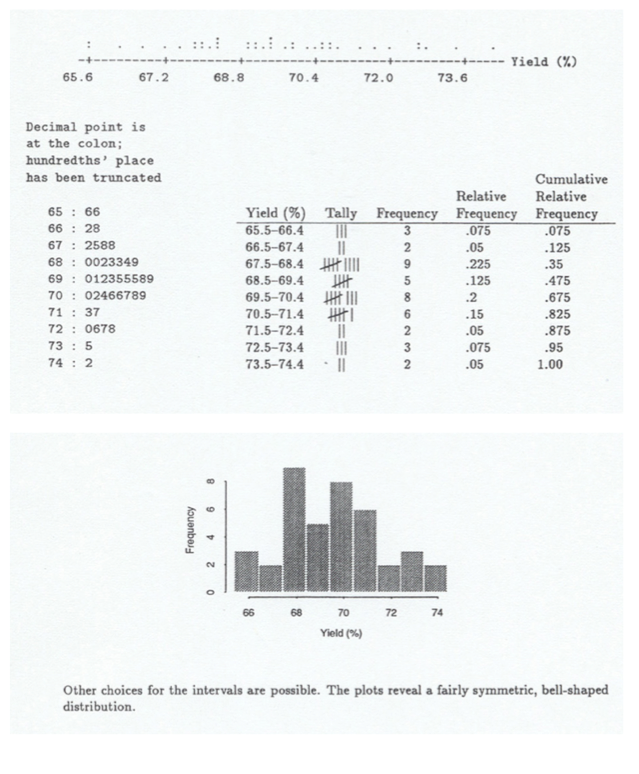
\includegraphics{../../fig/ch3s1p1sol.png}



\item Vardeman and Jobe Chapter 3 Section 2, part (a) of problem 1 (page 92):

\setkeys{Gin}{width=.75\textwidth} 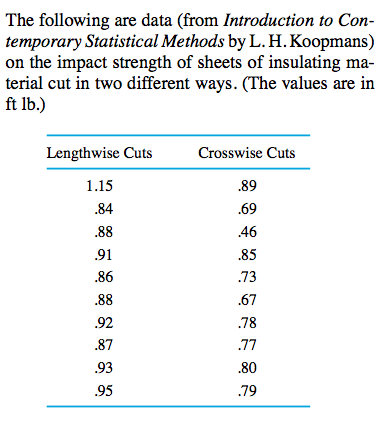
\includegraphics{../../fig/ch3s2p1.png}
Find the medians, quartiles, and the .37 quantiles of the two datasets.

\setkeys{Gin}{width=.75\textwidth} 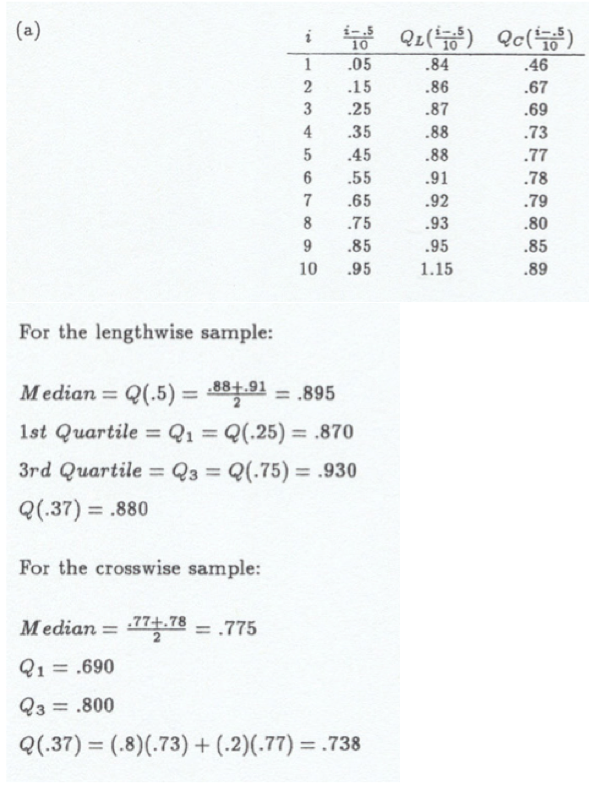
\includegraphics{../../fig/ch3s2p1sol.png}

\color{red}

You can read Q(0.25) and Q(0.75) directly from the table since $0.25$ and $0.75$ are each $\frac{i - 0.5}{10}$ for $i = 3$ and $i = 8$, respectively. And as I said in class, since there is an even number of observations for both the crosswise data and the lengthwise data, the median in each case is just the average of the middle two values. Hence, since $n = 10$ for both lists of numbers, we average $x_5$ and $x_6$ to get the median in each case. \q

For the lengthwise sample, here is how I calculate $Q(0.37)$. First, I pick $i' = np + 0.5 = 10 \cdot 0.37 + 0.5 = 4.2$. Then, I calculate Q(0.37) as follows:

\begin{align*}
Q(0.37) &= (\lceil i' \rceil - i') x_{\lfloor i' \rfloor} + ( i' - \lfloor i' \rfloor) x_{\lceil i' \rceil} \\
&= (\lceil 4.2 \rceil - 4.2) x_{\lfloor 4.2 \rfloor} + ( 4.2 - \lfloor 4.2 \rfloor) x_{\lceil 4.2 \rceil} \\
&= (5- 4.2) x_{4} + ( 4.2 - 4) x_{5} \\
&= (0.8) x_{4} + (0.2) x_{5} \\
&= (0.8)(0.88) + (0.2)(0.88) \\
&= 0.88
\end{align*}

For the crosswise sample, here is how I calculate $Q(0.37)$. As before, I pick $i' = np + 0.5 = 10 \cdot 0.37 + 0.5 = 4.2$. Then, I calculate Q(0.37) as follows:

\begin{align*}
Q(0.37) &= (\lceil i' \rceil - i') x_{\lfloor i' \rfloor} + ( i' - \lfloor i' \rfloor) x_{\lceil i' \rceil} \\
&= (\lceil 4.2 \rceil - 4.2) x_{\lfloor 4.2 \rfloor} + ( 4.2 - \lfloor 4.2 \rfloor) x_{\lceil 4.2 \rceil} \\
&= (5- 4.2) x_{4} + ( 4.2 - 4) x_{5} \\
&= (0.8) x_{4} + (0.2) x_{5} \\
&= (0.8)(0.73) + (0.2)(0.77) \\
&= 0.738
\end{align*}


\color{black}


\item Identify the following distributional shapes:

\setkeys{Gin}{width=.75\textwidth} 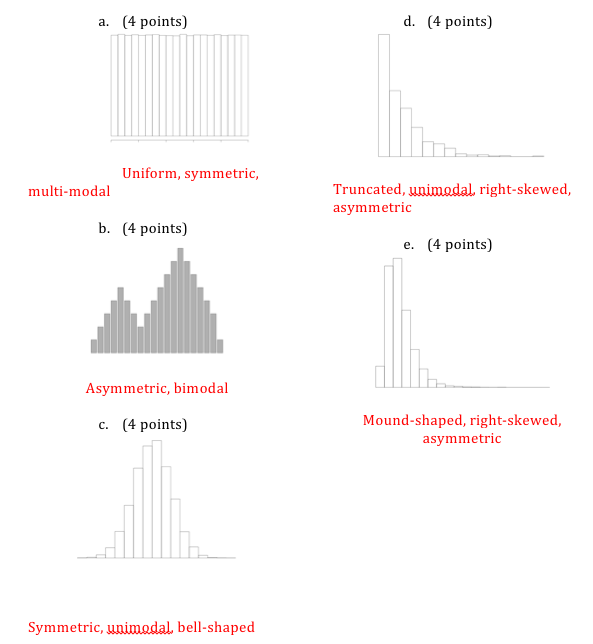
\includegraphics{../../fig/hw2shapessol.png}












\item Weekly feedback. You get full credit as long as you write something.
\begin{enumerate}[1. ]
\item Is there any aspect of the subject matter that you currently struggle with? If so, what specifically do you find difficult or confusing? The more detailed you are, the better I can help you.
{\color{red} You got full credit as long as you wrote something.}
\item Do you have any questions or concerns about the material, class logistics, or anything else? If so, fire away.
{\color{red} You got full credit as long as you wrote something.}
\end{enumerate}

\end{enumerate}




\end{flushleft}
%\newpage 
%\nocite{*}
%\bibliographystyle{plainnat} 
%\bibliography{}
\end{document}
